\comment{
In a database system, views are one of the central features in attaining both
logical data independence and efficient performance as evidenced by their use
from query optimization to data integration~\cite{halevy-vldbj01}. While
advances in view maintenance would have a significant impact on many database
internals challenges, our form of multilevel views and its realization as
efficient low-level code allows us to provide high-performance, lightweight
monitoring and notification services to the benefit of a wide range of
application domains. Consider the following applications:
}

Multilevel views and its realization as efficient low-level code
facilitates high-performance, lightweight monitoring for a wide range of
applications. Consider the following uses:

\vspace{-2mm}
\begin{list}{\labelenumi}{\usecounter{enumi} \leftmargin=1em}
\addtolength{\itemsep}{-0.5\baselineskip}
\item An automated stock market trading system monitors the distribution of buy
and sell orders of a particular stock to identify the best time and price for
its own orders.

\item A corporate data warehouse monitors its production facilities, warehoused
inventory and active demand for its products in order to identify
supply chain problems.

\item A compute cluster monitors its status to detect hardware failures
that place distributed tasks at risk of downtime.
\end{list}

\vspace{-1mm}
These uses require frontend analysis systems to drive rapid decision-making in
contrast to backend data warehouses for deep exploratory querying. These systems
sit on the critical datapath near data sources, and are key to a competitive
advantage. Query workloads are long-running and machine-generated, making the case for
incremental evaluation, and aggressive compilation and specialization over their
execution period. Other domains include regulatory
compliance~\cite{basel2}, scientific simulations~\cite{hey2009fourth}, and
disaster prediction~\cite{scholz1973earthquake}.


\vspace{1mm}
\tinysection{Query Workloads for Monitoring}
The above scenarios of algorithmic trading on order books, online
decision support at a manufacturer, and datacenter and network infrastructure
monitoring often involve computing a variety of statistics,
and comparing and contrasting them prior to taking action.
\comment{
Queries with complex dataflows consisting of nested and correlated subqueries
composed in arbitrary fashion abound.
}
Figure~\ref{fig:queries} lists the processing properties of a query workload
inspired by these domains that we use in this paper, with SQL code in
Appendix~\ref{app:queries}.

The algorithmic trading queries operate on two order book streams of a day's
worth of orders for the MSFT symbol on NASDAQ (approx. 2.5 million orders). The
online decision support queries are taken from the TPC-H and SSB benchmarks, and
processed over a randomized, replayed update stream.
\comment{The cluster monitoring query operates on a synthetic dataset that
simulates tasks running on a 20,000 node cluster.}
Our workload has a range of joins, predicates, and correlated
subqueries, up to depth 2. While a depth of 2 may seem low, we have not seen
many queries in popular DBMS benchmarks even approaching 4 or 5 nesting levels.

\begin{figure}[t]
\scriptsize{
\begin{center}
\begin{tabular}{ p{0.15cm} | l | c | c | c  | c }
\multicolumn{2}{c|}{}      & \#~Tables,  & Where- & Group- & \#~Subqueries\\
\multicolumn{2}{c|}{}      & join type.  & clause & bys    & and depth\\
\multicolumn{2}{c|}{Query} & =: equi     &        &        & \\
\multicolumn{2}{c|}{}      & x: cross    &        &        & \\
\hline
\begin{rotate}{90}\hspace{-1.1cm}Finance\end{rotate}
& AXF        & 2, =      & $\vee, <$     & yes & 0 / 0 \\
& BSP        & 2, =      & $\wedge, <$   & yes & 0 / 0 \\
& BSV        & 2, =      & None          & no  & 0 / 0 \\
& MST        & 2, x      & $\wedge, <$   & yes & 2 / 1 \\
& PSP        & 2, x      & $\wedge, <$   & no  & 2 / 1 \\
& VWAP       & 1         & $<$           & no  & 2 / 1
\vspace{0.5mm}
\\
\hline
\begin{rotate}{90}\hspace{-0.9cm}ETL\end{rotate}
& TPCH3      & 3, =      & $\wedge, <$   & yes & 0 / 0 \\
& TPCH11     & 2, =      & None          & yes & 0 / 0 \\
& TPCH17     & 2, =      & $<$           & no  & 1 / 1 \\
& TPCH18     & 3, =      & $<$           & yes & 1 / 2 \\
& TPCH22     & 1         & $=,<$         & yes & 2 / 1 \\
& SSB4       & 7, =      & $<$           & yes & 0 / 0 \\
\hline
\comment{
& SVL        & 1         & $\wedge, <$   & yes & 2 / 1 \\
}
\end{tabular}
\end{center}
}
\vspace{-4mm}
\caption{Features of the algorithmic trading, online decision support, and
cluster monitoring query workload used for experiments.}
\label{fig:queries}
\vspace{-3mm}
\end{figure}

The pertinent DBMS methods are triggers, and stream systems.
We benchmarked these queries on a mix of open-source and commercial stream
systems and DBMS (Esper, Postgres, CSPE, CDB)\footnote{We anonymize the
commercial systems due to licensing restrictions on publishing benchmarks.},
Figure~\ref{fig:enginecomp} shows their view refresh performance.
\comment{  
We describe implementation specifics below but defer further details such as
system configuration, to our in-depth experiments in
Section~\ref{sec:experiments}.
}
We do not include any native IVM results from commercial DBMS because despite
its wide availability, there are still many limitations on its usability.
In fact, none of the major DBMS supported incremental refresh for the
majority of our workload given the features in Figure~\ref{fig:queries}.
For many DBMS, the documented query
restrictions~\cite{db2-viewrestrict,mssql-viewrestrict,oracle-viewrestrict}
indicate that view materialization and maintenance cannot generally be applied
side-by-side with query optimization.
\comment{
This is a strong motivator for our goal of including materialization as a
first-class citizen in query optimization.
}

\vspace{1mm}
\tinysection{Triggers and Active Databases}
Trigger mechanisms facilitate the manipulation of database state in a reactive
manner, as DML statements execute.
The literature on triggers has focused on issues such as cascading, and
recursion, and to a lesser extent single-level IVM~\cite{baralis-rids95}.
Triggers can be implemented in a variety of languages from plpgsql, to Python or
C. For procedural SQL languages, triggers are compiled in the same way as
user-defined queries for interpretation by an executor.
\comment{
Triggers exemplify update processing where the developer looses the ability for
declarative development, and where along with user-defined functions and
aggregates, compilers and query optimizers reside in silos inside a DBMS.
}
This executor is designed for set-at-a-time computation rather than
fine-grained, pipelined computation. 

We implemented a \textit{repetitive} full refresh approach to maintain views for
our query workload, where after each update a trigger re-evaluates the query
from scratch.
\comment{
This approach incurs low developer overhead. Manually implementing
multilevel view maintenance is rapidly impractical after even one level of delta
rewriting due to code expansion, affirming the benefits of automatic
incrementalization during compilation.
}
Figure~\ref{fig:enginecomp} shows that for the small-state finance workload,
trigger performance does not vary across the types of queries. Here small-state
refers to the state accumulated while processing updates. In the finance
workload there are nearly as many deletes as inserts (unsuccessful orders are
often removed from the order books), and relations do not grow too large. For
large-state workloads, on Postgres, queries with nesting perform signficantly
worse than on CDB. Overall, CDB performs the best across all engines, primarily
with the mature optimizer in CDB choosing better plans and index usage.

\begin{figure}[t]
\vspace{-3mm}
\begin{center}
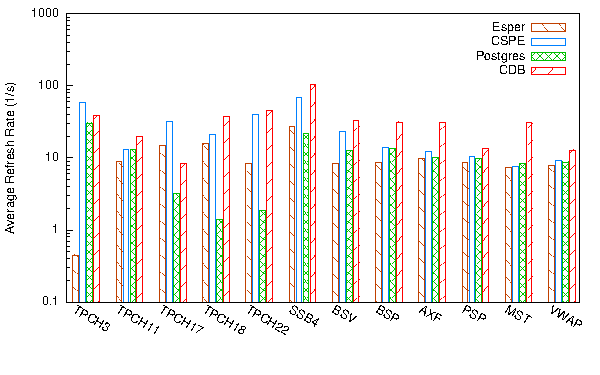
\includegraphics[scale=0.85]{../graphs/graphs/engine_bakeoff.pdf}
\end{center}
\vspace{-8mm}
\caption{A comparison of four stream systems and DBMS on full refresh view
maintenance.}
\label{fig:enginecomp}
\vspace{-4mm}
\end{figure}


\vspace{1mm}
\tinysection{Stream and Complex Event Processing}
These systems (SPEs) provide low-latency push-based processing and at first
glance may appear to be ideal for frontend analytics.
\comment{
However, in addition to
constructs such as windows or patterns and Kleene closure, monitoring
applications often have additional requirements -- they must often work with
long-lived, large state. This latter requirement is not well-addressed by
current SPEs, they rely on in-memory tables with suboptimal querying or
external DBMS access, and cannot support end-to-end incremental computation.
}
However, monitoring applications must often work with long-lived, large state,
and this requirement is not well-addressed by current SPEs. They either rely on
in-memory tables with suboptimal engines or external DBMS access, and do not
support incremental computation over large state.

Our implementation varied significantly across Esper and CSPE, due to a
clear lack of standardized semantics and portability across
SPEs~\cite{botan-pvldb:10,jain-pvldb:08}.
In both Esper and CSPE, we maintained indexed in-memory tables to represent base
relations, due to the inapplicability of windows to handle arbitrary updates and
deletes.
For Esper, we were unable to use subqueries in stream-to-table join operations,
which despite being supported in the language, resulted in differing,
inconsistent snapshots of tables that were used multiple times in a query (e.g.
self-joins), similar in effect to the state bug from
views~\cite{colby-sigmod:96}.
CSPE on the other hand did not support subqueries in stream-to-table operations.

On both systems, our approach performed stream-to-table joins to trigger the
replay of tables as streams via scans, as updates arrive. The replayed tables
were then processed by stream-only operators to implement fully pipelined plans.
\comment{
Our implementation strategy involved maintaining update streams as in-memory
tables, replaying relevant tables as updates arrive to turn tables into streams,
and wiring together stream operators to implement query plans. This essentially
constructs fully pipelined physical query plans and turns out to be very similar
to writing trigger code in procedural SQL languages once the stream is fully
replayed.
}
Additionally, we explicitly restricted both Esper and CSPE to single-threaded
execution and relied on their deterministic tuple processing order to avoid
complex locking and barriering to implement aggregate subqueries. We found such
serialization added substantial programming complexity and performance overheads
to our implementation.

Figure~\ref{fig:enginecomp} shows that for the finance workload, there is little
variation between Esper and CSPE, although CSPE does consistently outperform
Esper, but cannot match triggers in CDB. For the large-state queries, CSPE
outperforms Esper by significantly, and provides a viable alternative to
triggers in CDB with an overall lower variance in performance across both
nested (TPCH 17, 18, 22) and flat queries. Esper performs poorly on
TPCH 3 by missing index usage.
\comment{
Overall across all engines, we observed that index maintenance helped
significantly on the TPCH queries for a marginal maintenance cost.
}

The takeaway from these experiments is that with complex analysis workloads
involving nested queries and aggregate comparisons, SPEs often cannot take
advantage of the semantics they were designed for (e.g. windows, patterns), and
do not offer advantages over trigger processing. Furthermore neither system
achieves a high absolute refresh rate, of more than roughly 100 refreshes a
second suggesting limited responsiveness and poor scaling when considering many
simultaneous queries.

\tinysection{Other related work} In addition to the citations throughout this
paper, IBM's SPADE language~\cite{gedik-sigmod:08} has explored compilation and
fusion for stream queries, and Ghanem et
al.~\cite{DBLP:journals/tods/GhanemELA10} have presented a model for stream
processing with views. Neither of these consider as
general an incremental evaluation framework as provided by our multilevel views.
